

\tikzset{every picture/.style={line width=0.75pt}} %set default line width to 0.75pt        

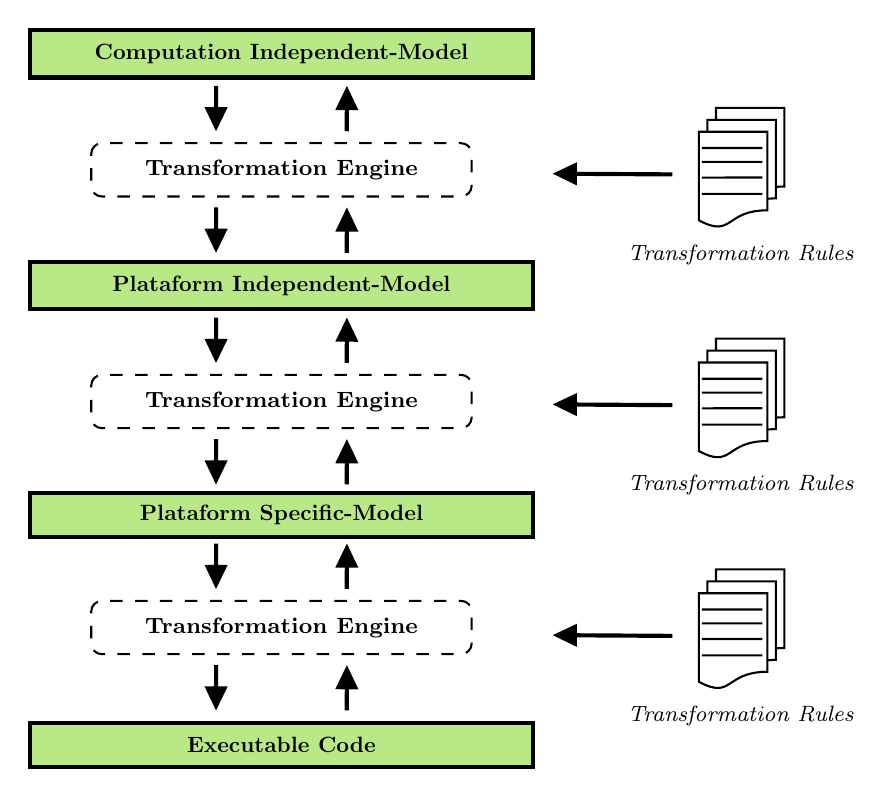
\begin{tikzpicture}[x=0.75pt,y=0.75pt,yscale=-1,xscale=1]
%uncomment if require: \path (0,442.3645935058594); %set diagram left start at 0, and has height of 442.3645935058594

%Shape: Rectangle [id:dp7655816759589134] 
\draw  [fill={rgb, 255:red, 184; green, 233; blue, 134 }  ,fill opacity=1 ][line width=1.5]  (52.59,47.21) -- (295.12,47.21) -- (295.12,70.24) -- (52.59,70.24) -- cycle ;

%Shape: Rectangle [id:dp37583246050722807] 
\draw  [fill={rgb, 255:red, 184; green, 233; blue, 134 }  ,fill opacity=1 ][line width=1.5]  (52.59,159.07) -- (295.12,159.07) -- (295.12,181.86) -- (52.59,181.86) -- cycle ;

%Shape: Rectangle [id:dp8974163182307999] 
\draw  [fill={rgb, 255:red, 184; green, 233; blue, 134 }  ,fill opacity=1 ][line width=1.5]  (52.59,270.24) -- (295.12,270.24) -- (295.12,291.66) -- (52.59,291.66) -- cycle ;

%Shape: Rectangle [id:dp7966059165934565] 
\draw  [fill={rgb, 255:red, 184; green, 233; blue, 134 }  ,fill opacity=1 ][line width=1.5]  (52.59,381.18) -- (295.12,381.18) -- (295.12,402.38) -- (52.59,402.38) -- cycle ;

%Straight Lines [id:da6759491853813937] 
\draw [line width=1.5]    (142.38,74.28) -- (142.34,93.11) ;
\draw [shift={(142.33,96.11)}, rotate = 270.14] [fill={rgb, 255:red, 0; green, 0; blue, 0 }  ][line width=1.5]  [draw opacity=0] (11.61,-5.58) -- (0,0) -- (11.61,5.58) -- cycle    ;

%Straight Lines [id:da4410578197502153] 
\draw [line width=1.5]    (205.33,96.11) -- (205.38,77.28) ;
\draw [shift={(205.39,74.28)}, rotate = 450.14] [fill={rgb, 255:red, 0; green, 0; blue, 0 }  ][line width=1.5]  [draw opacity=0] (11.61,-5.58) -- (0,0) -- (11.61,5.58) -- cycle    ;


%Rounded Rect [id:dp07358787233218322] 
\draw  [dash pattern={on 4.5pt off 4.5pt}][line width=0.75]  (82.21,106.98) .. controls (82.21,104.15) and (84.51,101.85) .. (87.35,101.85) -- (260.37,101.85) .. controls (263.2,101.85) and (265.5,104.15) .. (265.5,106.98) -- (265.5,122.4) .. controls (265.5,125.24) and (263.2,127.54) .. (260.37,127.54) -- (87.35,127.54) .. controls (84.51,127.54) and (82.21,125.24) .. (82.21,122.4) -- cycle ;

%Straight Lines [id:da6727844668924288] 
\draw [line width=1.5]    (142.38,132.84) -- (142.34,151.67) ;
\draw [shift={(142.33,154.67)}, rotate = 270.14] [fill={rgb, 255:red, 0; green, 0; blue, 0 }  ][line width=1.5]  [draw opacity=0] (11.61,-5.58) -- (0,0) -- (11.61,5.58) -- cycle    ;

%Straight Lines [id:da05695276066757793] 
\draw [line width=1.5]    (205.33,154.67) -- (205.38,135.84) ;
\draw [shift={(205.39,132.84)}, rotate = 450.14] [fill={rgb, 255:red, 0; green, 0; blue, 0 }  ][line width=1.5]  [draw opacity=0] (11.61,-5.58) -- (0,0) -- (11.61,5.58) -- cycle    ;


%Straight Lines [id:da5342535617428192] 
\draw [line width=1.5]    (142.38,185.91) -- (142.34,204.74) ;
\draw [shift={(142.33,207.74)}, rotate = 270.14] [fill={rgb, 255:red, 0; green, 0; blue, 0 }  ][line width=1.5]  [draw opacity=0] (11.61,-5.58) -- (0,0) -- (11.61,5.58) -- cycle    ;

%Straight Lines [id:da815215430339091] 
\draw [line width=1.5]    (205.33,207.74) -- (205.38,188.91) ;
\draw [shift={(205.39,185.91)}, rotate = 450.14] [fill={rgb, 255:red, 0; green, 0; blue, 0 }  ][line width=1.5]  [draw opacity=0] (11.61,-5.58) -- (0,0) -- (11.61,5.58) -- cycle    ;


%Rounded Rect [id:dp7817143384899228] 
\draw  [dash pattern={on 4.5pt off 4.5pt}][line width=0.75]  (82.21,218.61) .. controls (82.21,215.78) and (84.51,213.47) .. (87.35,213.47) -- (260.37,213.47) .. controls (263.2,213.47) and (265.5,215.78) .. (265.5,218.61) -- (265.5,234.03) .. controls (265.5,236.86) and (263.2,239.16) .. (260.37,239.16) -- (87.35,239.16) .. controls (84.51,239.16) and (82.21,236.86) .. (82.21,234.03) -- cycle ;

%Straight Lines [id:da45101461047602665] 
\draw [line width=1.5]    (142.38,244.47) -- (142.34,263.3) ;
\draw [shift={(142.33,266.3)}, rotate = 270.14] [fill={rgb, 255:red, 0; green, 0; blue, 0 }  ][line width=1.5]  [draw opacity=0] (11.61,-5.58) -- (0,0) -- (11.61,5.58) -- cycle    ;

%Straight Lines [id:da05505279480496861] 
\draw [line width=1.5]    (205.33,266.3) -- (205.38,247.47) ;
\draw [shift={(205.39,244.47)}, rotate = 450.14] [fill={rgb, 255:red, 0; green, 0; blue, 0 }  ][line width=1.5]  [draw opacity=0] (11.61,-5.58) -- (0,0) -- (11.61,5.58) -- cycle    ;


%Straight Lines [id:da8230912155193482] 
\draw [line width=1.5]    (142.38,294.79) -- (142.34,313.62) ;
\draw [shift={(142.33,316.62)}, rotate = 270.14] [fill={rgb, 255:red, 0; green, 0; blue, 0 }  ][line width=1.5]  [draw opacity=0] (11.61,-5.58) -- (0,0) -- (11.61,5.58) -- cycle    ;

%Straight Lines [id:da4013158878484284] 
\draw [line width=1.5]    (205.33,316.62) -- (205.38,297.79) ;
\draw [shift={(205.39,294.79)}, rotate = 450.14] [fill={rgb, 255:red, 0; green, 0; blue, 0 }  ][line width=1.5]  [draw opacity=0] (11.61,-5.58) -- (0,0) -- (11.61,5.58) -- cycle    ;


%Rounded Rect [id:dp7359504066475293] 
\draw  [dash pattern={on 4.5pt off 4.5pt}][line width=0.75]  (82.21,327.5) .. controls (82.21,324.66) and (84.51,322.36) .. (87.35,322.36) -- (260.37,322.36) .. controls (263.2,322.36) and (265.5,324.66) .. (265.5,327.5) -- (265.5,342.91) .. controls (265.5,345.75) and (263.2,348.05) .. (260.37,348.05) -- (87.35,348.05) .. controls (84.51,348.05) and (82.21,345.75) .. (82.21,342.91) -- cycle ;

%Straight Lines [id:da8028685074596458] 
\draw [line width=1.5]    (142.38,353.35) -- (142.34,372.18) ;
\draw [shift={(142.33,375.18)}, rotate = 270.14] [fill={rgb, 255:red, 0; green, 0; blue, 0 }  ][line width=1.5]  [draw opacity=0] (11.61,-5.58) -- (0,0) -- (11.61,5.58) -- cycle    ;

%Straight Lines [id:da3923230440168086] 
\draw [line width=1.5]    (205.33,375.18) -- (205.38,356.35) ;
\draw [shift={(205.39,353.35)}, rotate = 450.14] [fill={rgb, 255:red, 0; green, 0; blue, 0 }  ][line width=1.5]  [draw opacity=0] (11.61,-5.58) -- (0,0) -- (11.61,5.58) -- cycle    ;


%Straight Lines [id:da9965571371249939] 
\draw [line width=1.5]    (362.2,116.9) -- (307.59,116.57) ;
\draw [shift={(304.59,116.55)}, rotate = 360.35] [fill={rgb, 255:red, 0; green, 0; blue, 0 }  ][line width=1.5]  [draw opacity=0] (11.61,-5.58) -- (0,0) -- (11.61,5.58) -- cycle    ;

%Flowchart: Multidocument [id:dp4462030708787881] 
\draw  [fill={rgb, 255:red, 255; green, 255; blue, 255 }  ,fill opacity=1 ] (383.22,84.88) -- (416.2,84.88) -- (416.2,122.73) .. controls (395.59,122.73) and (399.71,136.38) .. (383.22,127.55) -- cycle ; \draw  [fill={rgb, 255:red, 255; green, 255; blue, 255 }  ,fill opacity=1 ] (379.09,90.61) -- (412.08,90.61) -- (412.08,128.46) .. controls (391.46,128.46) and (395.59,142.11) .. (379.09,133.28) -- cycle ; \draw  [fill={rgb, 255:red, 255; green, 255; blue, 255 }  ,fill opacity=1 ] (374.97,96.35) -- (407.96,96.35) -- (407.96,134.2) .. controls (387.34,134.2) and (391.46,147.85) .. (374.97,139.02) -- cycle ;
%Straight Lines [id:da3428056744320267] 
\draw    (376.37,104.19) -- (405.55,104.18) ;


%Straight Lines [id:da737270903434551] 
\draw    (376.37,110.9) -- (405.55,110.89) ;


%Straight Lines [id:da8869180718660374] 
\draw    (376.37,118.42) -- (405.55,118.4) ;


%Straight Lines [id:da4672287889638409] 
\draw    (376.37,126.31) -- (405.55,126.29) ;




%Straight Lines [id:da01844945320814495] 
\draw [line width=1.5]    (362.2,228.07) -- (307.59,227.74) ;
\draw [shift={(304.59,227.72)}, rotate = 360.35] [fill={rgb, 255:red, 0; green, 0; blue, 0 }  ][line width=1.5]  [draw opacity=0] (11.61,-5.58) -- (0,0) -- (11.61,5.58) -- cycle    ;

%Flowchart: Multidocument [id:dp3024584461272144] 
\draw  [fill={rgb, 255:red, 255; green, 255; blue, 255 }  ,fill opacity=1 ] (383.22,196.05) -- (416.2,196.05) -- (416.2,233.9) .. controls (395.59,233.9) and (399.71,247.55) .. (383.22,238.72) -- cycle ; \draw  [fill={rgb, 255:red, 255; green, 255; blue, 255 }  ,fill opacity=1 ] (379.09,201.78) -- (412.08,201.78) -- (412.08,239.64) .. controls (391.46,239.64) and (395.59,253.29) .. (379.09,244.45) -- cycle ; \draw  [fill={rgb, 255:red, 255; green, 255; blue, 255 }  ,fill opacity=1 ] (374.97,207.52) -- (407.96,207.52) -- (407.96,245.37) .. controls (387.34,245.37) and (391.46,259.02) .. (374.97,250.19) -- cycle ;
%Straight Lines [id:da8403992079487277] 
\draw    (376.37,215.36) -- (405.55,215.35) ;


%Straight Lines [id:da6998171999275149] 
\draw    (376.37,222.07) -- (405.55,222.06) ;


%Straight Lines [id:da5741349416674424] 
\draw    (376.37,229.59) -- (405.55,229.57) ;


%Straight Lines [id:da07308866987359197] 
\draw    (376.37,237.48) -- (405.55,237.46) ;




%Straight Lines [id:da3151258876682197] 
\draw [line width=1.5]    (362.2,339.24) -- (307.59,338.91) ;
\draw [shift={(304.59,338.89)}, rotate = 360.35] [fill={rgb, 255:red, 0; green, 0; blue, 0 }  ][line width=1.5]  [draw opacity=0] (11.61,-5.58) -- (0,0) -- (11.61,5.58) -- cycle    ;

%Flowchart: Multidocument [id:dp028531838068365012] 
\draw  [fill={rgb, 255:red, 255; green, 255; blue, 255 }  ,fill opacity=1 ] (383.22,307.22) -- (416.2,307.22) -- (416.2,345.07) .. controls (395.59,345.07) and (399.71,358.72) .. (383.22,349.89) -- cycle ; \draw  [fill={rgb, 255:red, 255; green, 255; blue, 255 }  ,fill opacity=1 ] (379.09,312.95) -- (412.08,312.95) -- (412.08,350.81) .. controls (391.46,350.81) and (395.59,364.46) .. (379.09,355.62) -- cycle ; \draw  [fill={rgb, 255:red, 255; green, 255; blue, 255 }  ,fill opacity=1 ] (374.97,318.69) -- (407.96,318.69) -- (407.96,356.54) .. controls (387.34,356.54) and (391.46,370.19) .. (374.97,361.36) -- cycle ;
%Straight Lines [id:da3021760556251445] 
\draw    (376.37,326.53) -- (405.55,326.52) ;


%Straight Lines [id:da14331632044731157] 
\draw    (376.37,333.24) -- (405.55,333.23) ;


%Straight Lines [id:da17482156708678565] 
\draw    (376.37,340.76) -- (405.55,340.75) ;


%Straight Lines [id:da025053397684865253] 
\draw    (376.37,348.65) -- (405.55,348.63) ;





% Text Node
\draw (173.86,58.72) node [scale=0.8] [align=left] {\textbf{Computation Independent-Model}};
% Text Node
\draw (173.86,170.46) node [scale=0.8] [align=left] {\textbf{Plataform Independent-Model}};
% Text Node
\draw (173.86,280.95) node [scale=0.8] [align=left] {\textbf{Plataform Specific-Model}};
% Text Node
\draw (173.86,391.78) node [scale=0.8] [align=left] {\textbf{Executable Code}};
% Text Node
\draw (173.86,114.69) node  [align=left] {{\footnotesize \textbf{Transformation Engine}}};
% Text Node
\draw (173.86,226.32) node  [align=left] {{\footnotesize \textbf{Transformation Engine}}};
% Text Node
\draw (173.86,335.2) node  [align=left] {{\footnotesize \textbf{Transformation Engine}}};
% Text Node
\draw (395.59,155.53) node  [align=left] {{\footnotesize \textit{Transformation Rules}}};
% Text Node
\draw (395.59,266.71) node  [align=left] {{\footnotesize \textit{Transformation Rules}}};
% Text Node
\draw (395.59,377.88) node  [align=left] {{\footnotesize \textit{Transformation Rules}}};


\end{tikzpicture}
